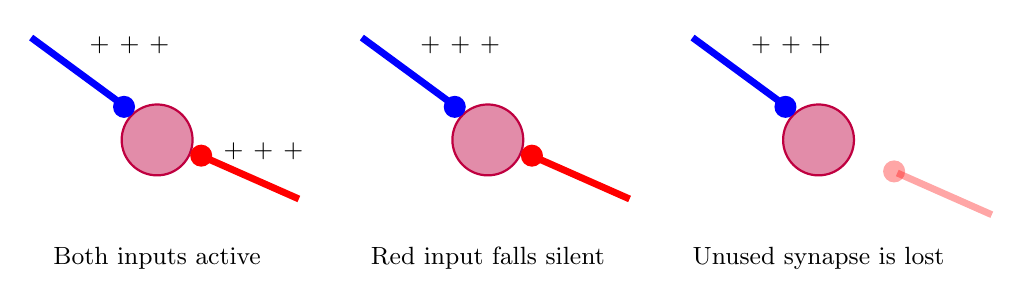
\begin{tikzpicture}[font=\small]
% panel 1: both inputs active
\begin{scope}[shift={(0,0)}]
  \fill[purple, fill opacity=0.45] (0,0) circle (0.45);
  \draw[purple, thick] (0,0) circle (0.45);
  \draw[blue, line width=2.5pt] (-1.6,1.3) -- (-0.47,0.47);
  \fill[blue] (-0.42,0.42) circle (0.14);
  \node at (-0.35,1.2) {$+\,+\,+$};
  \draw[red, line width=2.5pt] (1.8,-0.75) -- (0.6,-0.22);
  \fill[red] (0.56,-0.2) circle (0.14);
  \node at (1.35,-0.15) {$+\,+\,+$};
  \node[align=center] at (0,-1.5) {Both inputs active};
\end{scope}
% panel 2: red input silent
\begin{scope}[shift={(4.2,0)}]
  \fill[purple, fill opacity=0.45] (0,0) circle (0.45);
  \draw[purple, thick] (0,0) circle (0.45);
  \draw[blue, line width=2.5pt] (-1.6,1.3) -- (-0.47,0.47);
  \fill[blue] (-0.42,0.42) circle (0.14);
  \node at (-0.35,1.2) {$+\,+\,+$};
  \draw[red, line width=2.5pt] (1.8,-0.75) -- (0.6,-0.22);
  \fill[red] (0.56,-0.2) circle (0.14);
  \node[align=center] at (0,-1.5) {Red input falls silent};
\end{scope}
% panel 3: silent synapse withdrawn
\begin{scope}[shift={(8.4,0)}]
  \fill[purple, fill opacity=0.45] (0,0) circle (0.45);
  \draw[purple, thick] (0,0) circle (0.45);
  \draw[blue, line width=2.5pt] (-1.6,1.3) -- (-0.47,0.47);
  \fill[blue] (-0.42,0.42) circle (0.14);
  \node at (-0.35,1.2) {$+\,+\,+$};
  \draw[red, line width=2.5pt, opacity=0.35] (2.2,-0.95) -- (1.0,-0.42);
  \fill[red, opacity=0.35] (0.96,-0.4) circle (0.14);
  \node[align=center] at (0,-1.5) {Unused synapse is lost};
\end{scope}
\end{tikzpicture}
